
As previously discussed in Section~\ref{subsec:qcd}, the detection of quarks is indirect due to quark confinement.
The hadronization processes manifest in the detector as a shower of hadrons. Using clustering algorithms, these hadronic showers can be reconstructed as a cone-shaped energy pattern, known as a jet.


\subsection{Small-R jet selection}
\label{subsec:jet_selection}

When a heavy particle decays, it can produce two quarks that rapidly move away from each other, leading to the formation of two distinct jets of particles in the detector. If the decaying particle is moving slowly, the resulting jets tend to be more compact and easily distinguishable. These compact jets, characterized by a smaller radius parameter (R) in their clustering algorithm, are referred to as Small-R jets.

Small-R jets are used for reconstructing the less boosted $W/Z \to qq$ candidates, identifying \(qq\) pairs from \(V\) boson decays as ``Signal'' jets and forward jets in vector-boson scattering as ``VBS'' jets. Sections \ref{subsec:vbs_selection} and \ref{subsubsec:merged_jets_selection}-\ref{subsubsec:resolved_jets_selection} provide in-depth discussions on Signal and VBS jets. We use the ATLAS baseline jet reconstruction algorithm, the \texttt{AntiKt4EMPFlowJets}, which is anti-$k_t$ clustering algorithm~\cite{Cacciari_2008}.
Standard jet calibrations are implemented, including the use of Jet Vertex Tagging (JVT) with a Medium Working Point (WP) to reduce pile-up interactions~\cite{ATLAS-CONF-2014-018}.
Pile-up interactions refer to the multiple, simultaneous collisions of other proton pairs occurring alongside the primary collision event.
To further suppress pile-up jets, especially in the forward-like topology relevant to our analysis, the forward-JetVertexTagger (fJVT)~\cite{ATL-PHYS-PUB-2019-026} is applied, enhancing the focus on jets from the targeted VBS processes.
Small-R jet selection criteria is summarized in Table~\ref{tab:small_R_jet_summary}.

\begin{table}[ht]
\caption{Summary of Selection Criteria and Calibration Methods for Small-R Jets}
\label{tab:small_R_jet_summary}
\resizebox{0.95\textwidth}{!}{
\begin{tabular}{|c|c|c|}
\hline
%\large
\multicolumn{3}{|c|}{Jet Reconstruction Parameters} \\
%\normalsize
\hline
Parameter & \multicolumn{2}{c|}{Value} \\ 
\hline
algorithm & \multicolumn{2}{c|}{anti-k$_\text{T}$}  \\
R-parameter & \multicolumn{2}{c|}{0.4} \\
input constituent & \multicolumn{2}{c|}{EMPFlow} \\
Analysis Release Number &\multicolumn{2}{c|}{ 21.2.164 } \\
%CalibArea tag & \multicolumn{2}{c|}{00-04-82} \\
%Calibration configuration & \multicolumn{2}{c|}{JES\_MC16Recommendation\_Consolidated\_PFlow\_Apr2019\_Rel21.config} \\
Calibration sequence (Data) & \multicolumn{2}{c|}{JetArea\_Residual\_EtaJES\_GSC\_Insitu} \\
Calibration sequence (MC) & \multicolumn{2}{c|}{JetArea\_Residual\_EtaJES\_GSC\_Smear} \\
%Calibration sequence (AFII) & JetArea\_Residual\_EtaJES\_GSC \\
\hline
%\large
\multicolumn{3}{|c|}{Selection Requirements} \\
%\normalsize
\hline
%& \textbf{``Signal'' jet} & \textbf{``VBS'' jet} \\
%\hline
Observable & \multicolumn{2}{c|}{Requirement} \\
\hline
Jet cleaning & \multicolumn{2}{c|}{LooseBad} \\
\hline
BatMan cleaning & \multicolumn{2}{c|}{Yes} \\
\hline
\pt                         & \multicolumn{2}{c|}{$>$20~GeV ($|\eta|<2.5$) and $>$30~GeV ($2.5<|\eta|<4.5$)}   \\
\hline
\textbar$\eta$\textbar      & \multicolumn{2}{c|}{$<4.5$} \\
\hline
JVT & \multicolumn{2}{c|}{$>0.5$ for 60 GeV$<\pt<$120~GeV and $\left|\eta\right|<2.4$ } \\
WP  & \multicolumn{2}{c|}{Medium} \\
%Config  & \multicolumn{2}{c|}{Moriond2018/JvtSFFile\_EMPFlow.root} \\
\hline
fJVT & \multicolumn{2}{c|}{$>0.5$ (and $|timing|<10 \ ns$)} \\
     & \multicolumn{2}{c|}{for $\pt<$120~GeV and $2.5 < \left|\eta\right|<4.5$}  \\
WP   & \multicolumn{2}{c|}{Loose} \\
%Config  & \multicolumn{2}{c|}{Moriond2018/fJvtSFFile.root} \\
\hline
$b$-tagging (See Sec.~\ref{subsec:flavortagging}) & \multicolumn{2}{c|}{Tagged, or not tagged} \\
\hline
\end{tabular}}
\end{table}






\clearpage
\subsection{Large-R jet selection}
\label{subsec:large-Rjet}
For high-\pt $W/Z \to qq$ candidates, the angle between the two jets narrows, leading to the merging of jets, as shown in Figure~\ref{fig:jet_merging}. Clustering algorithms then reconstruct them into a single, larger-radius jet, known as a large-R jet, which contains the two merged sub-jets.
Following the trimming procedure\cite{Krohn:2009th} to reduce pile-up and soft radiation effects, the ``jet mass'', $m_J$, 
is reconstructed by summing the four-vectors of jet constituents. The large-R jets then undergo baseline kinematic cuts:

        \begin{itemize}
                \item $\pt^{J} > 200 \, \GeV$
                \item $|\eta|^{J} < 2$
                \item $m^{J} > 50 \, \GeV$
        \end{itemize}

The (large-R) jet substructure variable, $D_{2}$, derived from the energy correlation functions based on energies and pair-wise angles of the sub-constituents\cite{Larkoski:2014gra,Larkoski:2015kga}, is sensitive to the expected 2-prong sub-structure from the boosted W/Z bosons decay. The variable $D_{2}$ is defined as
\begin{equation}
D^{(\beta=1)}_2 = E_{CF3} \left( \frac{E_{CF1}}{E_{CF2}} \right)^3 \\
\end{equation}
where the energy correlation functions ($E_{CF}$) are defined as:
\begin{equation}
\begin{aligned}
E_{CF1} &= \sum_{i} p_{T,i} \\
E_{CF2} &= \sum_{ij} p_{T,i}p_{T,j} \Delta R_{ij} \\
E_{CF3} &= \sum_{ijk} p_{T,i}p_{T,j}p_{T,k} \Delta R_{ij} \Delta R_{jk} \Delta R_{ki}
\end{aligned}
\end{equation}

The track multiplicity, $n_{\text{Tracks}}$, of the ungroomed large-R jet is also used to enhance background rejection. It is particularly sensitive to QCD jets from single-quark and gluon decays. 
%The utilization of these variables in defining the merged category is detailed in Section~\ref{subsubsec:merged_jets_selection}.
The $W/Z$ boson tagger, based on three variables—$m_J$, $D_{2}$, $n_{\text{Tracks}}$—is used to identify boson jets from large-R jet candidates. The application of this tagger and the three variables in defining the merged category is elaborated in Section~\ref{subsubsec:merged_jets_selection}.

\begin{figure}[htbp]
    \centering
    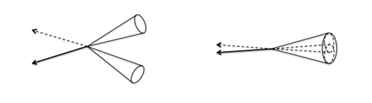
\includegraphics[width=0.65\textwidth]{figures/object_definition/jet_merging.png}
    \caption{Illustration of jets merging}
    \label{fig:jet_merging}
\end{figure}

%%%
Summary of selections and calibrations of the large-R jet is shown in Table~\ref{tab:largeR_jet_summary}.


\begin{table}[ht]
\caption{Summary of Selection Criteria and Calibration Methods for Large-R Jet}
\label{tab:largeR_jet_summary}
\resizebox{0.95\textwidth}{!}{
\begin{tabular}{|c|c|}
\hline
%\large
\multicolumn{2}{|c|}{Jet Reconstruction Parameters} \\
\hline
%\normalsize
Parameter & Value \\ 
\hline
algorithm & anti-k$_{T}$  \\
R-parameter & 1.0 \\
input constituent & LCTopoCluster \\
grooming algorithm & Trimming \\ 
$f_{cut}$ & 0.05 \\
$R_{trim}$ & 0.2 \\
Analysis Release Number & 21.2.164 \\
%Calibration tag & JetCalibTools-00-04-76 \\
%CalibArea tag & 00-04-81 \\
%Calibration configuration (Data) & JES\_MC16recommendation\_FatJet\_Trimmed\_JMS\_comb\_March2021.config \\
%Calibration configuration (MC) & JES\_MC16recommendation\_FatJet\_Trimmed\_JMS\_comb\_17Oct2018.config \\
Calibration sequence (Data) & EtaJES\_JMS\_Insitu\_InsituCombinedMass \\
Calibration sequence (MC) & EtaJES\_JMS \\
\hline
%\large
\multicolumn{2}{|c|}{Selection Requirements} \\
%\normalsize
\hline
Observable & Requirement \\
\hline
\pt  & $>$200 GeV \\
\textbar$\eta$\textbar & $<$2.0 \\
mass & $>$ 50~GeV \\
\hline
\multicolumn{2}{|c|}{SmoothedWZTagger} \\\hline
Object  & Working point \\\hline
$W$/$Z$ & 3-var tagger working point \\
%$Z\rightarrow bb$ & single/double b-tag with/without loose/tight mass \\\hline
%        & \texttt{SmoothedContainedVTagger\_AntiKt10LCTopoTrimmed\_FixedSignalEfficiencyXX\_MC16\_20201216.dat} \\
        & with V = {W, Z} and XX = {50, 80} \\
\hline
\end{tabular}}
\end{table}


